\section{Derivadas}

\subsection{Primeras definiciones}

\begin{definicion}
	  La \emph{derivada} de $y=f(x)$ en el punto $x$ está definida como
	\begin{align*}
		f'(x)= \lim_{h\to 0}\dfrac{f(x+h)-f(x)}{h}
		= \lim_{\Delta x \to 0}\dfrac{\Delta y}{\Delta x}
	\end{align*}

	donde $h=\Delta x$, $\Delta y=f(x+h)-f(x)=f(x+\Delta x)-f(x)$ siempre que tal límite exista.
\end{definicion}

\begin{observacion}
	Si $\Delta x \approx 0$ y $f'(x)$ existe, entonces
	\begin{align*}
		\Delta y \approx f'(x) \Delta x.
	\end{align*}
	En física, el diferencial de $x$ es un cambio \emph{infinitesimal}  en dicha variable.
\end{observacion}


%%%%%%%%%%%%%%%%%%%%%
{}
  \begin{definicion}
   Si $y = f(x)$ y $f'(x)$ existe, el diferencial de $y$ está dado por
   \begin{align*}
    dy = f'(x)dx
    \end{align*}
  \end{definicion}


%%%%%%%%%%%%%%%%%%%%%
{}
  El proceso de encontrar las derivadas de una función se conoce como \emph{diferenciación}.

%%%%%%%%%%%%%%%%%%%%%
{}
  \begin{definicion}[Derivadas de alto orden]
   \begin{align*}
    \dfrac{d^{n}y}{dx^{n}}=
    \begin{cases}
f(x) & n=0 \\
\dfrac{d}{dx}\left( \dfrac{d^{n-1}}{dx^{n-1}}f(x) \right) & n>0
\end{cases}
    \end{align*}
  \end{definicion}


%%%%%%%%%%%%%%%%%%%%%
{}
  Usualmente rescribimos
  \begin{align*}
   y' = \dfrac{dy}{dx} \\
   y'' = \dfrac{d^{2}y}{dx^{2}}
   \end{align*}

   En el caso $n>2$, es más común escribir
 $   y^{(n)}$ para denotar a la $n-$ésima derivada.

%%%%%%%%%%%%%%%%%%%%%
\subsection{Interpretación geométrica}
  Geométricamente, la derivada $f'(a)$ de una función $f(x)$, en un punto dado $x=a$, representa \emph{pendiente de la recta tangente} a $y=f(x)$ en el punto $\left( a,f(a) \right)$.

%%%%%%%%%%%%%%%%%%%%%
\subsection{Relación con continuidad}

  Si una función tiene derivada en un punto, entonces es continua en dicho punto.
  Sin embargo, el recíproco no es necesariamente cierto.

  \begin{resuelto}
	Demuestra que la función de valor absoluto $ f(x) = \sqrt{x^2}, x\in \R $ es continua en toda la recta real, pero no tiene derivada en $ x=0 $.
  \end{resuelto}

%%%%%%%%%%%%%%%%%%%%%
\subsection{Fórmulas de derivación}
{}
  En lo subsecuente, $u,v$ representarán funciones de $x$, mientras que $a,c,p$ representarán constantes.


  \emph{Supondremos que las derivadas de $u$ y $v$ existe, es decir, que son diferenciables}.

%%%%%%%%%%%%%%%%%%%%%
{}
  \begin{figure}
 \centering
 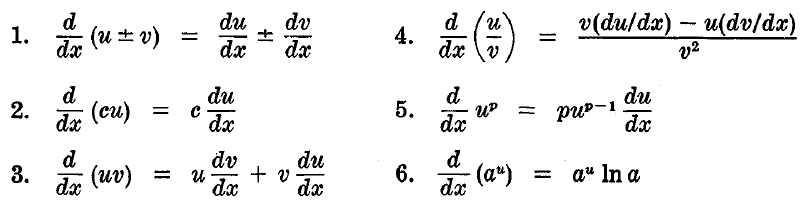
\includegraphics[width=.7\textwidth,keepaspectratio=true]{./calculo/formulas_derivadas_01.png}
 % formulas_derivadas_01.png: 810x220 px, 96dpi, 21.43x5.82 cm, bb=0 0 607 165
 \caption{Fórmulas usuales de derivadas}
 \label{fig:formulas_derivadas_01}
\end{figure}


%%%%%%%%%%%%%%%%%%%%%
{}
  \begin{figure}
 \centering
 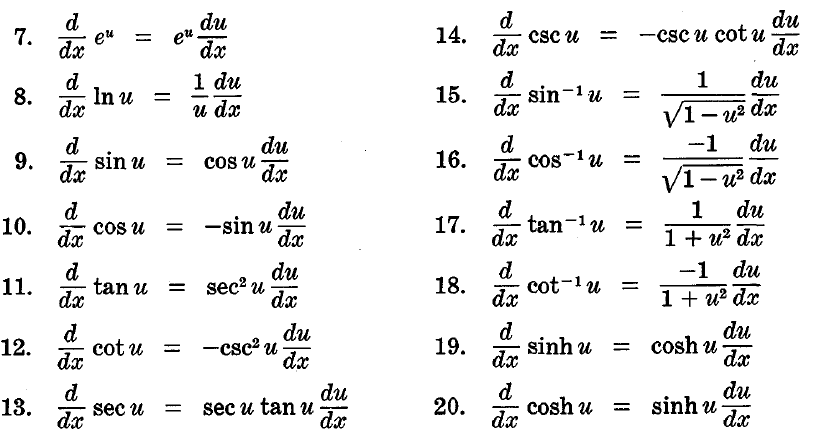
\includegraphics[width=.7\textwidth,keepaspectratio=true]{./calculo/formulas_derivadas_02.png}
 % formulas_derivadas_01.png: 810x220 px, 96dpi, 21.43x5.82 cm, bb=0 0 607 165
 \caption{Fórmulas usuales de derivadas}
 \label{fig:formulas_derivadas_02}
\end{figure}


%%%%%%%%%%%%%%%%%%%%%
{}
  En particular, cuando $u=x$, las fórmulas se simplifican porque $\dfrac{du}{dx}=1$.

%%%%%%%%%%%%%%%%%%%%%
  \begin{resuelto}
   Demostrar que si $u$ y $v$ son funciones diferenciables
   \begin{enumerate}[(i)]
     %NUEVO ITEM
     \item \[\dfrac{d}{dx}\left( u+v \right) =
     \dfrac{du}{dx}+\dfrac{dv}{dx}\]

     \item \[\dfrac{d}{dx}\left( uv \right) = u\dfrac{dv}{du}+v\dfrac{du}{dx}
     \]
\end{enumerate}
  \end{resuelto}


%%%%%%%%%%%%%%%%%%%%%
{}
  \begin{resuelto}
   Demostrar que si $f(x)$ tiene una derivada en $x=a$, entonces $f(x)$ es continua en $x=a$.
  \end{resuelto}


%%%%%%%%%%%%%%%%%%%%%
{}
  \begin{resuelto}
   Demostrar que si $p$ es cualquier entero positivo, y $u$ es una función diferenciable respecto a $x$, entonces
   \begin{align*}
    \dfrac{d}{dx}u^{p}=pu^{p-1}\dfrac{du}{dx}
    \end{align*}
  \end{resuelto}


%%%%%%%%%%%%%%%%%%%%%
{}